\problemname{Iguana Honeymoon
}

\intextsep2mm
\begin{wrapfigure}{r}{50mm}
 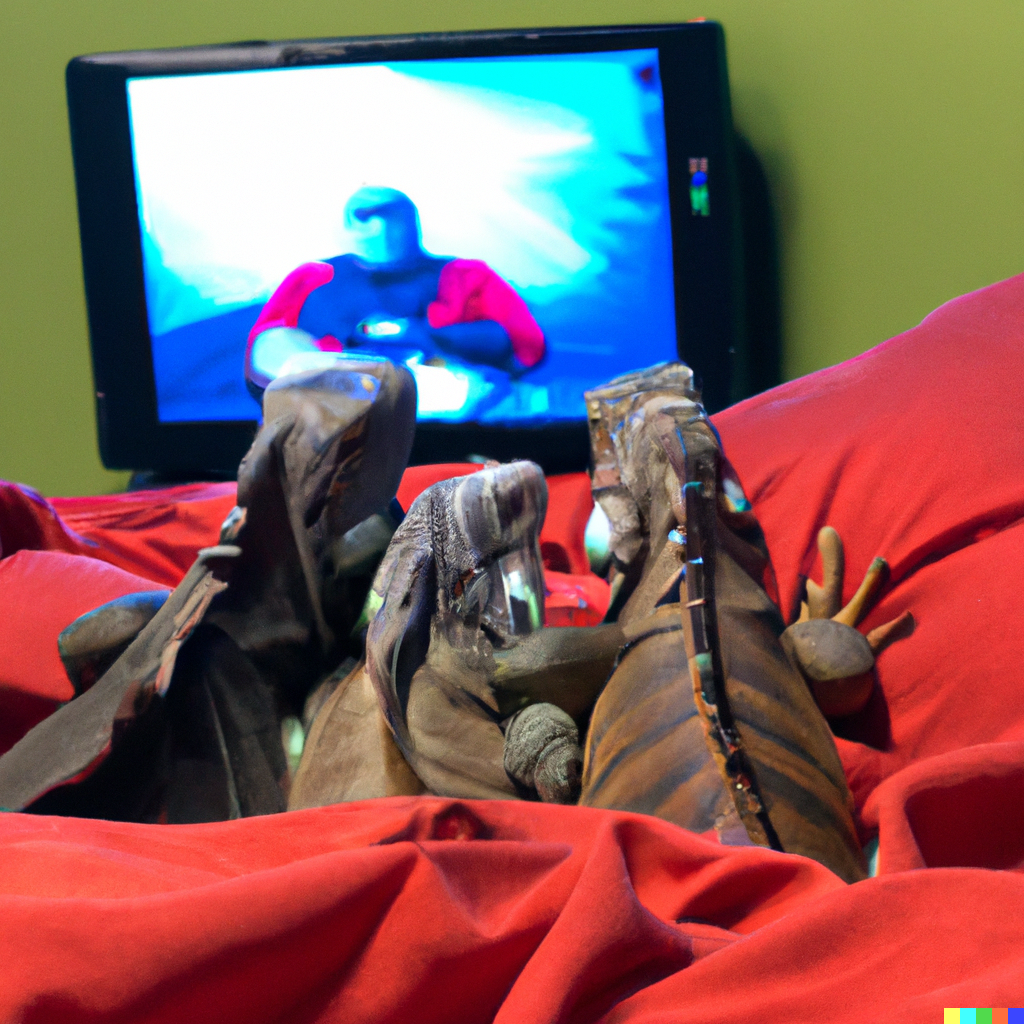
\includegraphics[width=50mm]{img.png}
\end{wrapfigure}
~

The legendary iguanas Izzy and Iggy just got married and are heading to their honeymoon. The newlyweds are working on picking a movie to `watch' during their honeymoon. Izzy really likes movies about cats and/or pirates. Iggy really likes movies about pirates and/or skeletons. As such, during each scene of a movie, Izzy is interested if the scene is about cats or pirates and is very interested if the scene is about cats and pirates. Similarly, Iggy is interested if the scene is about pirates or skeletons and is very interested if the scene is about both.

Izzy and Iggy enjoy watching movies together but prefer scenes where they are both equally interested (either both very interested, both interested, or both not interested).

Can you help Izzy and Iggy pick the movie that has the most scenes where Izzy and Iggy would be equally interested?


\section*{Input}

The first line of input contains a single integer $N$~($1 \leq N \leq 100$), which is the number of movies Izzy and Iggy are considering.

Then, $N$ movie descriptions follow. Each movie description starts with a line containing a string of uppercase letters $T_i$~($1 \leq |T_i| \leq 100$), which is the title of movie $i$, and an integer $M_i$~($1 \leq M \leq 100$), which is the number of scenes in the movie. The following $M_i$ lines describe the scenes in movie $i$. Each of these lines contains three strings that are either \texttt{Y} or \texttt{N} (shortened versions of `yes' and `no'). The first string says whether or not this scene is about cats, the second says if the scene is about pirates, and the third says if the scene is about skeletons.

No two movies have the same title.


\section*{Output}

Display the title of the movie that has the most scenes where Izzy and Iggy would be equally interested. If there are multiple such movies, choose the title that comes lexicographically first.

